\documentclass[main.tex]{subfiles}

\begin{document}

\renewcommand{\labelitemi}{\ding{226}}
\renewcommand{\labelitemii}{\ding{227}}

\part{ND280 upgrade}
\label{pt:up}

\chapter{Introduction}
\label{ch:up:motif}
As mentioned in \autoref{ch:T2K:general}, the first goal of the T2K experiment was to measure the $\theta_{13}$ mixing angle. After the successful discovery of the $\theta_{13}$, T2K entered a phase of the precise measurement of the neutrino oscillation parameters. The experiment provides the most precise estimations for the $\theta_{23}$ angle and also very accurate measurements of the $\Delta m_{23}$ and $\theta_{13}$ parameters. Great progress was obtained in the search for the CP--violation with the determination of the 3$\sigma$ confidence level on the possible values of the $\delta_{CP}$~\cite{Abe2020n}. The $\delta_{CP}$ measurement became the main goal of the experiment.

The next-generation experiments like DUNE~\cite{Acciarri2016} and Hyper-Kamiokande~\cite{Proto-Collaboration2018} will be able to achieve 3$\sigma$ sensitivity to the CP--violation across the wide range of the $\delta_{CP}$ values but on the time scale 2026 and beyond. The T2K experiment can probe this effect with less sensitivity but much earlier. The sensitivity of the T2K experiment with the total statistics of $20\times10^{21}$ POT is shown in \autoref{fig:up:sens}.

\begin{figure}[!ht]
  \centering
  \begin{minipage}{0.49\linewidth}
    \centering
    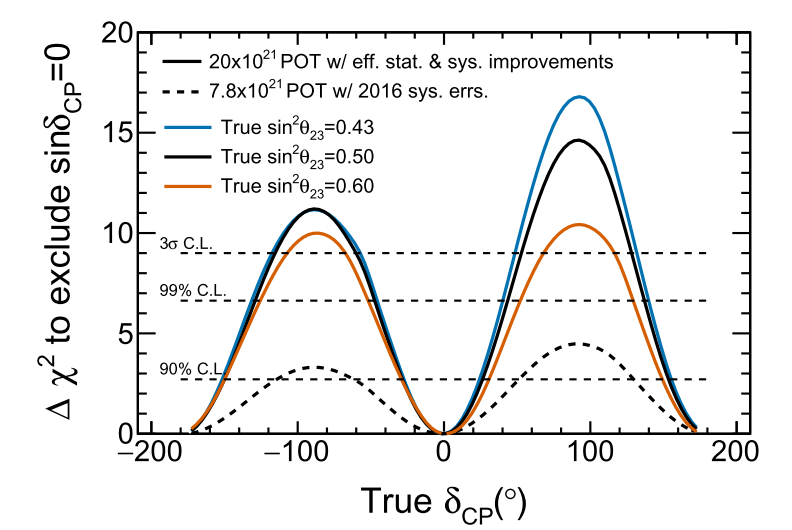
\includegraphics[width = \linewidth]{t2kII_dcp} \\ (a)
  \end{minipage}
  \begin{minipage}{0.49\linewidth}
    \centering
    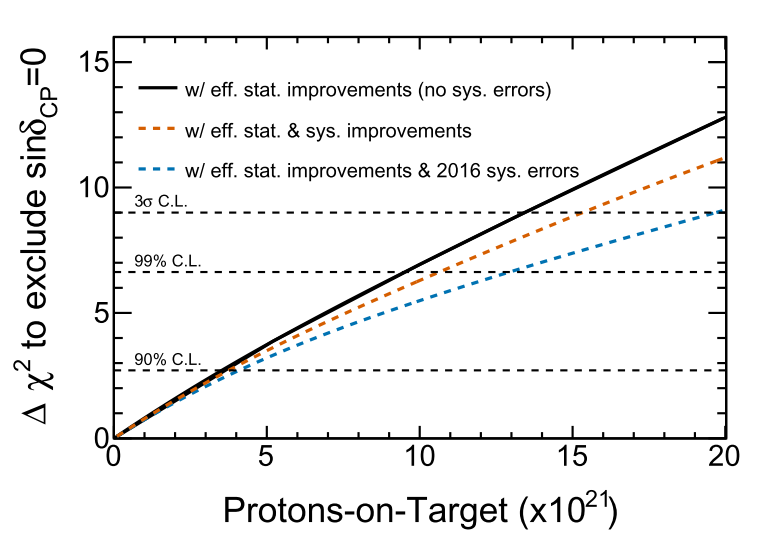
\includegraphics[width = \linewidth]{t2k_cp} \\ (b)
  \end{minipage}
    \caption{An expected sensitivity of the T2K experiment to the CP--violation in the neutrino oscillations. The known mass order is assumed. Three systematic uncertainties estimations are used: (blue) 2016 value, (orange) with improvements by factor 2/3 and (black) only stat. uncertainties. (a) shows the sensitivity over the $\delta_{CP}$ value and (b) shows the sensitivity evolution over the collected statistics for $\delta_{CP}=-\pi/2$.}
    \label{fig:up:sens}
\end{figure}


More statistics is necessary to determine the CP--violation more precisely and to justify if the effect takes place. The improvement of the sensitivity versus the collected data is shown in \autoref{fig:up:sens} b. Initially, T2K was supposed to collect the total statistics of $7.8\times10^{21}$ POT. The extended run of the T2K experiment aiming at the total statistics $20\times20^{21}$ POT was proposed~\cite{Abe2016e}. This additional period of data collection was called T2K-II. The beamline will be upgraded to provide a more intense neutrino beam (\autoref{sec:up:beam}). Therefore the data statistics accumulation will go faster.

There is a room for further improvement of the sensitivity with the reduction of the systematic uncertainty. \autoref{fig:up:sens} presents the sensitivity of the T2K experiment with different assumptions: current systematic uncertainties (in blue), improved systematics by factor 2/3 (in orange), only statistical uncertainty (in black). With the improved systematics, the desired sensitivity will be reached faster, and finally, a wider range of the $\delta_{CP}$ can be studied. The budget of the systematic uncertainties of the T2K experiment is described in~\cite{Abe2017}. The main sources in decreasing order are neutrino cross-sections, flux, secondary interactions in the SK, SK detector. The systematics related to the SK is very hard to reduce and it is going to be extremely expensive. Also, it gives a minor impact. The systematic uncertainty related to the neutrino cross-section and flux can be better constrained with the upgrade of the near detector.

T2K near detector provides good systematics reduction. It decreases the uncertainty of the oscillation analysis from 12\% down to 6\%. But for the T2K-II the further systematics reduction is required. To do this, several limitations of ND280 should be overcome. Originally ND280 was designed for the reconstruction of the forward-going particles, while the far detector Super-Kamiokande detects the particles in the $4\pi$ phase space. Also, ND280 is not able to detect low energy nucleons produced in the neutrino interactions that make the neutrino energy reconstruction inaccurate. The upgrade of the near detector is proposed (\autoref{sec:up:nd}). The idea is to use a highly granular target to reduce the threshold of particle detection. Above and below this target two new TPCs will be placed. Thus the phase space acceptance will be enlarged and include particles pointed in the perpendicular direction with respect to the incoming neutrino. With the improvements mentioned above the systematic uncertainty of the oscillation analysis will go below 4\%. The present value is about 6\%. Hence the improvement of the sensitivity illustrated in \autoref{fig:up:sens} is possible.


\section{Beamline upgrade}
\label{sec:up:beam}
Neutrino interactions are extremely rare processes. The natural way to gain statistics in the experiment is to use a very intense beam. The T2K experiment uses the beam produced by the J-PARC accelerator complex. After the few upgrades, the power of the beam in the main ring of the accelerator reached 500 kW. As a result, the J-PARC complex provides one of the most intense neutrino beams in the world. It was proved that T2K can obtain better physics results with the statistics extension to $20\times10^{21}$ POT~\cite{Abe2016e}. For this purpose, the J-PARC accelerator will be upgraded to provide an even more intense beam with the power of 1.3 MW.

\begin{figure}[!ht]
  \centering
  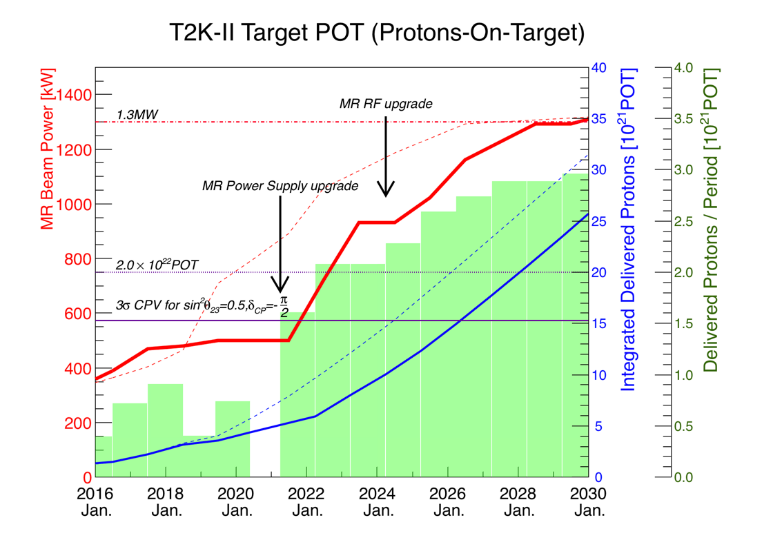
\includegraphics[width=0.6\linewidth]{beam_plan}
  \caption{Target J-PARC beam power (red) and the expected total accumulated statistics (blue) as a function of the year. Two possible schedules are considered shown with solid and dashed lines.}
  \label{fig:up:beam_plan}
\end{figure}

The beamline power upgrade schedule is shown in \autoref{fig:up:beam_plan}. The accelerator will be stopped for one year for the major hardware improvement. In the following years, the intensity will slightly grow alongside the data collection. The target power 1.3 MW is planned to be reached by 2028. This is beyond T2K. The Hyper-Kamiokande experiment is going to use the same beamline and use all the benefits from the power upgrade after the T2K. The details about the beamline upgrade are described in~\cite{Abe2019h}.

\section{Detector overview}
\label{sec:up:nd}


\subsection{Current detector limitations}
The T2K off-axis near detector is described in \autoref{sec:T2K:nd280} of \autoref{ch:T2K:general}. The schematic view of the setup is presented in \autoref{fig:T2K:ND280} (b). There are several known problems that limit the performance of the ND280. As a result, the total T2K systematics is dominated by the neutrino cross-section and flux uncertainty. These uncertainties can be reduced with better constraints with the upgraded ND280.

One of the main issues is limited phase-space coverage. An event display of a neutrino interaction in the ND280 as well as the detector layout is shown in \autoref{fig:up:ed_fgd1}. The scintillator neutrino targets (Fine Grained Detectors) are shown in violet. They are alternated with 3 TPCs shown in blue. Such a setup is perfect for the reconstruction of the forward and backward going particles. But if the lepton from the neutrino interaction goes at a high angle w.r.t. the beam (up/down in \autoref{fig:up:ed_fgd1}) we will not be able to perform accurate measurements. It will not leave a long enough track in the TPCs, hence we can not estimate the momentum with the curvature and the particle type with the energy loss. It is even possible that the particle goes alone the single vertical bar in FGD. In this case, even tracking with the scintillator detector is impossible. The efficiency of the muon selection from the $\nu_\mu CC$ interactions in the FGD1 over the outgoing lepton angle is shown in \autoref{fig:up:cos_eff_current}.

The far detector can detect the outgoing lepton with uniform efficiency over the 4$\pi$ phase-space. But the near detector can measure only neutrino interactions producing forward going leptons. The comparison of the detectors' acceptance and the expected lepton phase space are shown in \autoref{fig:up:ps}. To extend the constraints from the ND280 to the full phase-space various models of the neutrino interactions are used. But the uncertainties of such models are quite high. The direct measurements of the leptons in 4$\pi$ angle in the near detector will reduce the systematic uncertainty.

\begin{figure}[!ht]
  \centering
  \begin{minipage}{0.49\linewidth}
      \begin{flushleft}
      \begin{minipage}{0.9\linewidth}
      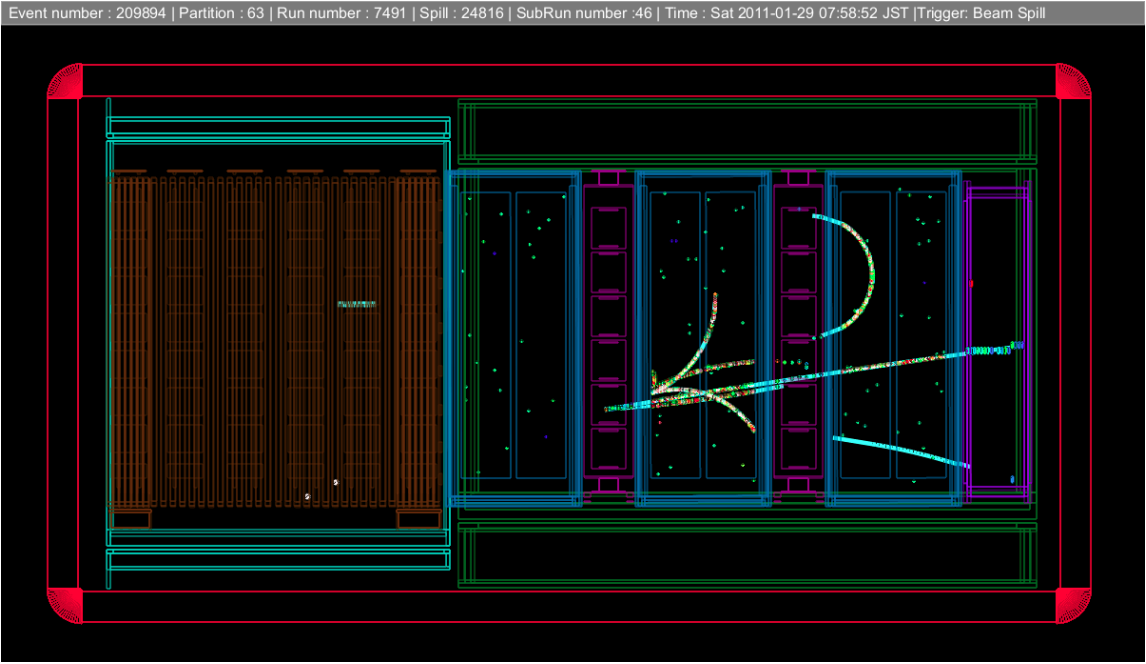
\includegraphics[width=\linewidth]{ed_fgd1}
      \caption{The event display of the neutrino interaction in the FGD1 in the ND280. The beam is coming from the left.}
      \label{fig:up:ed_fgd1}
      \end{minipage}
      \begin{minipage}{0.1\linewidth}
      \end{minipage}
      \end{flushleft}
  \end{minipage}
  \begin{minipage}{0.49\linewidth}
      \begin{flushright}
      \begin{minipage}{0.1\linewidth}
      \end{minipage}
      \begin{minipage}{0.9\linewidth}
      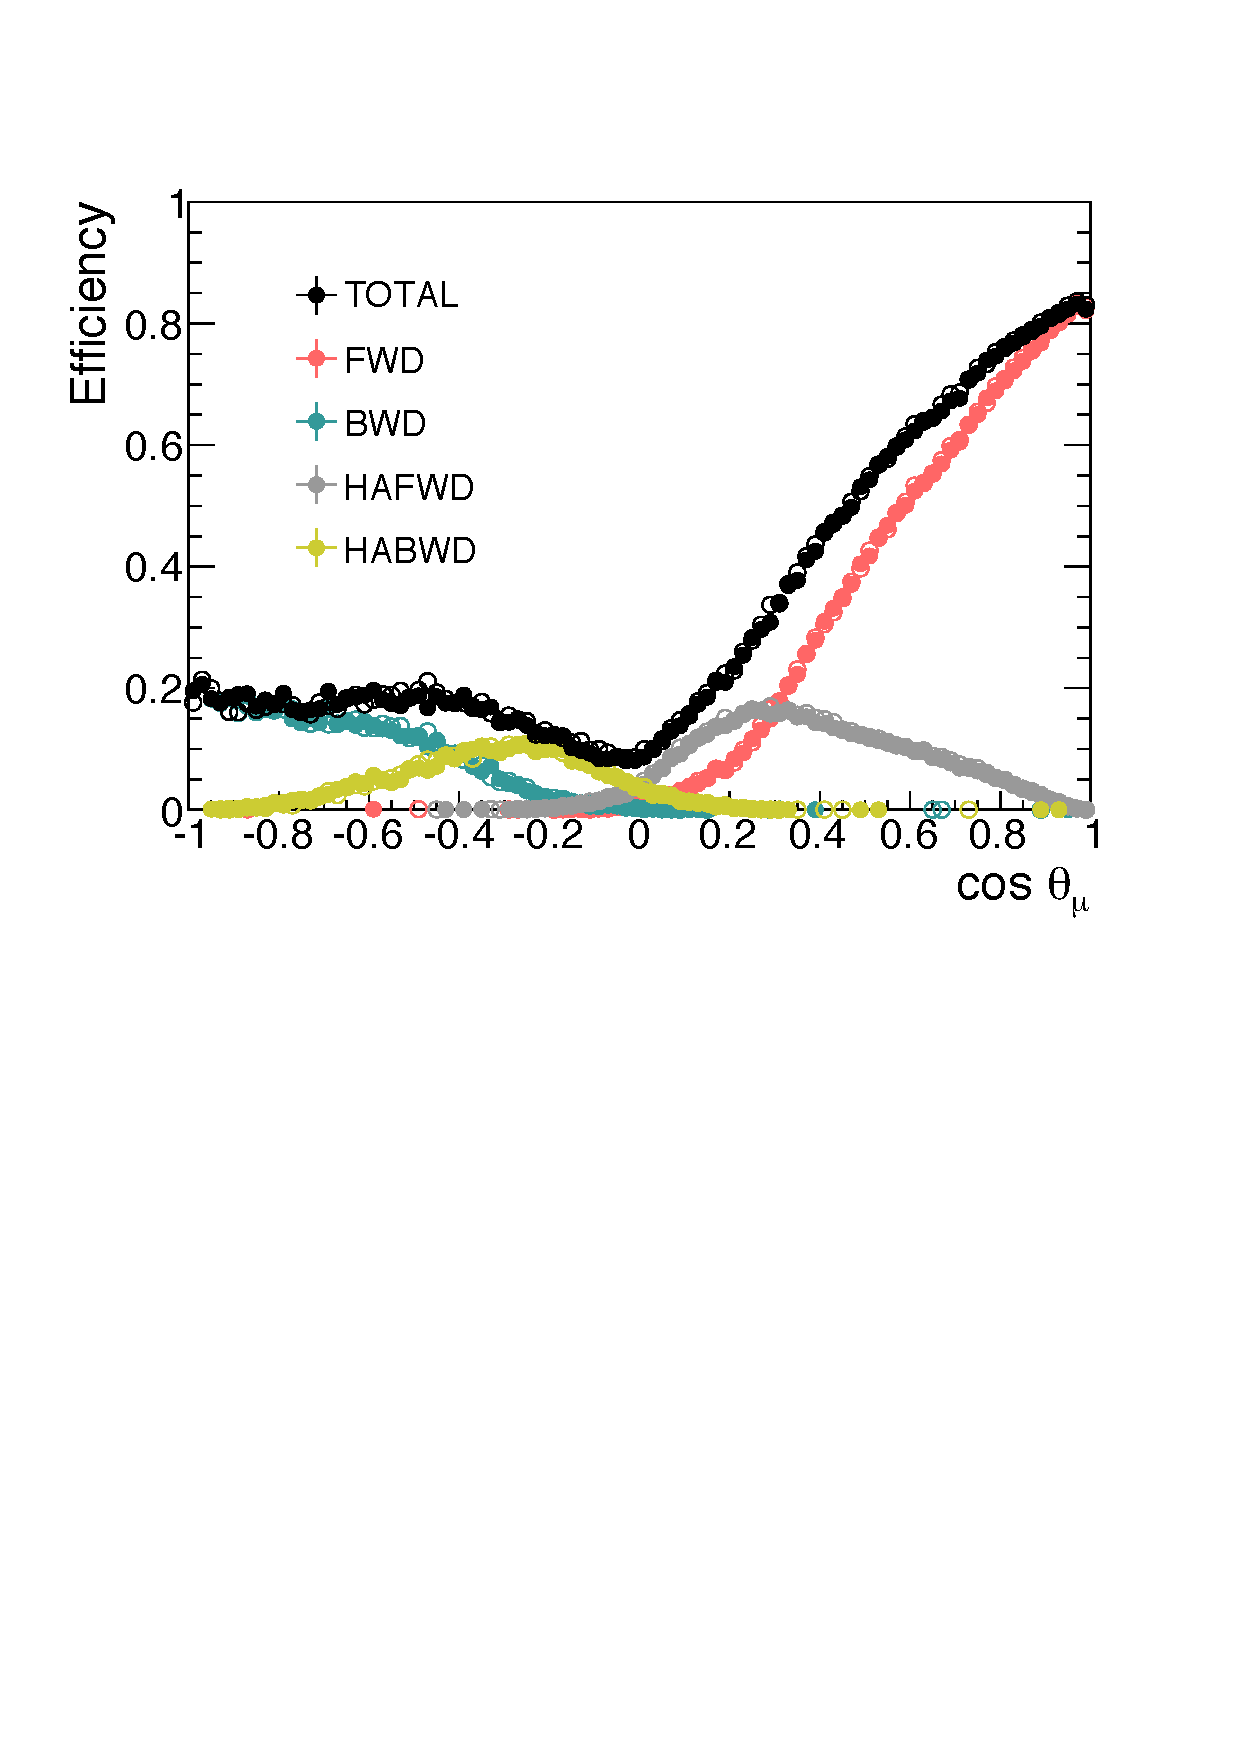
\includegraphics[width=\linewidth]{cos_eff_current}
      \caption{Muon selection efficiency from the $\nu_\mu CC$ interactions in the FGD1 as a function of the lepton angle w.r.t. Z axis.}
      \label{fig:up:cos_eff_current}
      \end{minipage}
      \end{flushright}
  \end{minipage}
\end{figure}

\begin{figure}[!ht]
  \centering
  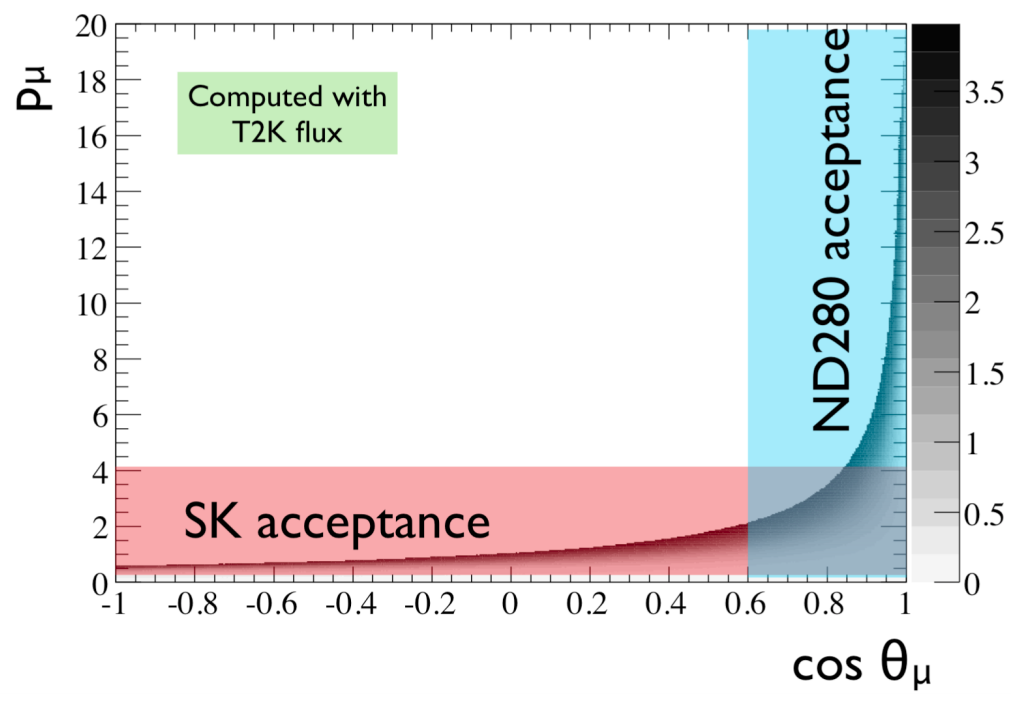
\includegraphics[width=0.5\linewidth]{nd_sk}
  \caption{The acceptance of both near and far detectors of the T2K experiment over the expected lepton phase space.}
  \label{fig:up:ps}
\end{figure}


The other subject of concern is the threshold of particle detection. Thanks to muon penetration ability, they are leaving a long track and can be easily detected. But protons from the neutrino interactions are mostly low energetic and travel a short distance. It's quite difficult to detect them with the sandwich scintillator detector like FGD. The proton should go through at least a few layers for robust detection. If it is pointing at a high angle w.r.t. beam the situation is even worse. The current threshold of the proton detection in FGDs is around 500 MeV, while the proton spectrum starts from 200 MeV. Nucleon detection from the neutrino interaction is extremely important in the T2K. As mentioned in \autoref{ch:T2K:general}, Super--Kamiokande uses CCQE interaction assumption to reconstruct the neutrino energy. But in most of the cases, neutrino doesn't interact with the free nucleon but with Oxygen nuclei in SK and with Carbon and Oxygen nuclei in ND280. The nuclear effects (\autoref{sec:intro:nuclei} of \autoref{ch:nu_phys}) are biasing the neutrino energy measurements. They can even change the event topology. For example, after neutrino interacts with pion production, the pion can be absorbed in the nuclei and the event will look like the CCQE interaction. That's why nuclear effects should be precisely constrained. It can be done with the precise measurement of both outgoing lepton and nucleon kinematics. The detection of short pion tracks will also help with the proper reconstruction of the interaction topology and will gain the neutrino energy estimation accuracy as well.

\subsection{New design proposal}

To improve the performance of the near detector its upgrade was proposed~\cite{Abe2019}. The ND280 tracker (2 FGDs and 3 TPCs) will be kept in place and will continue operation. Thus the data from both T2K-I and T2K-II can be analyzed together. The $\pi^0$ detector will be replaced with the new neutrino target and 2 horizontal TPCs. The upstream part will be surrounded by the time of flight (ToF) detectors. The various CAD models are presented in \autoref{fig:up:nd_up} and \autoref{fig:up:nd_cad}.

\begin{figure}[!ht]
  \centering
  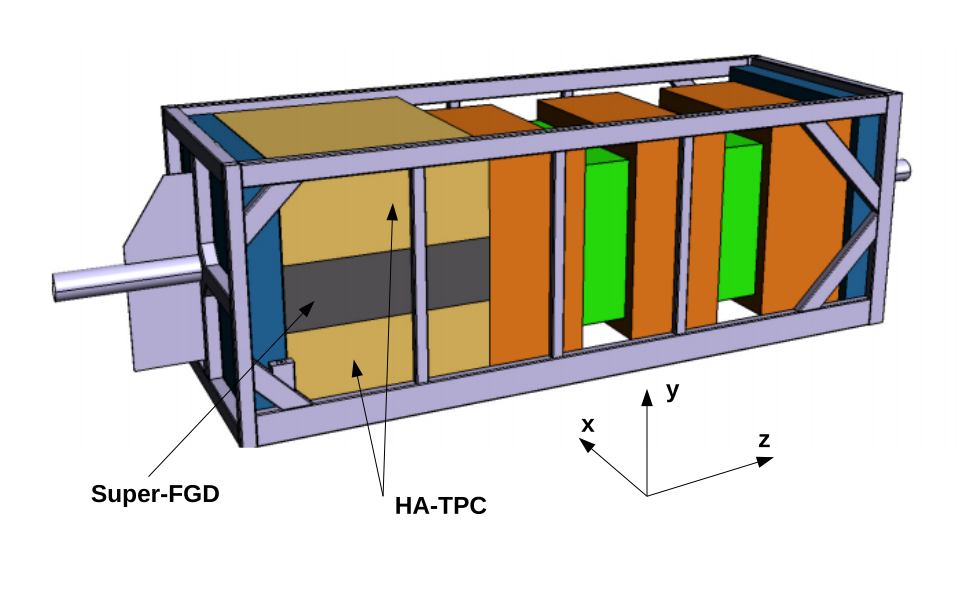
\includegraphics[width=0.5\linewidth]{nd_up}
  \caption{The scheme of the upgraded near detector. The downstream part is kept as it is. The new horizontal target and two high angle TPCs are put in the upstream part,}
  \label{fig:up:nd_up}
\end{figure}

\begin{figure}[!ht]
  \centering
  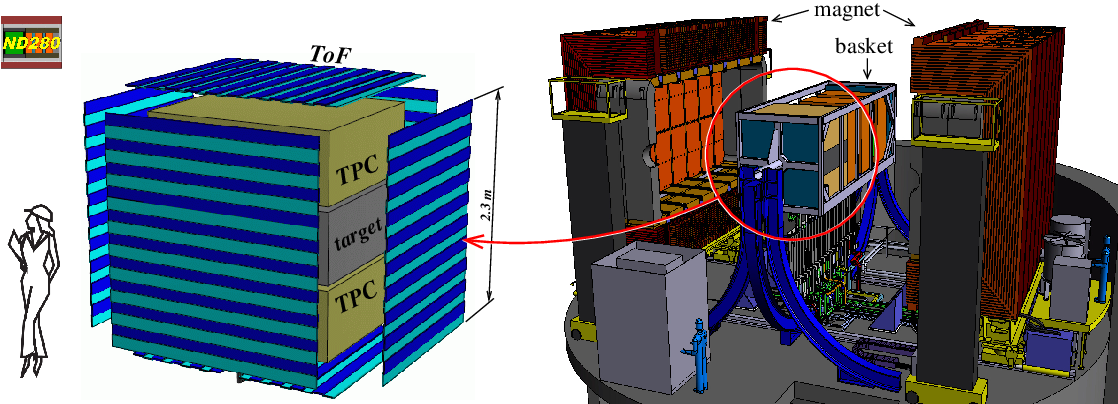
\includegraphics[width=\linewidth]{nd_CAD}
  \caption{The CAD model of the whole upgraded detector setup and the inset of the mostly affected by the modifications upstream part.}
  \label{fig:up:nd_cad}
\end{figure}

The new neutrino target Super-FGD (SFGD) will be composed of small plastic scintillator cubes. The cube edge is set to 1 cm providing fine granularity. Three orthogonal holes are drilled in the cube for the light readout with the WLS fibers. Therefore the Super-FGD can reconstruct the tracks in 3D. High granularity significantly reduces the threshold of particle tracking. Also, such a structure will improve the separation between gamma conversion and electron neutrino CC interaction resulting in more precise $\nu_e$ cross-section measurements. The dimensions of the new target are $182\times184\times56 \text{ cm}^3$ giving a total mass close to 2 tonnes. The total fiducial mass of the ND280 will be nearly doubled. The large size of the target allows detecting the secondary interactions of the neutrons from the anti-neutrino CCQE interactions $\overline{\nu}+p\to\ell+n$. As mentioned in the \nameref{ch:up:motif} measurement of the outgoing nucleons are critical for the precise neutrino energy reconstruction and probing neutrino interactions models. The details of the neutron detection proposal are presented in \autoref{ch:up:neutron}. More details about SFGD detector will be provided in \autoref{ch:up:sfgd}.

Two atmospheric pressure High angle TPCs (HATPC) will be put above and below Super-FGD. They will enlarge the phase space to the full coverage. The readout will be organized by the Micromegas (MM) as for the current TPC, but new technology will be implemented. The Micromegas will be covered with the resistive foil resulting in charge spreading over the pads. Thus the spatial resolution can be improved with the same pad size. It will lead to better momentum reconstruction and finally more accurate neutrino energy estimations. The details about HATPC detector will be provided in \autoref{ch:up:tpc}.

The Time of Flight (ToF) detectors will fully cover the upstream part of the ND280. It will be composed of scintillator bars and readout with the MPPC arrays. This detector will help with the reconstruction of the particle direction: to/from Super-FGD. Neutrino interacts quite often in the magnet coil and ECal and can produce a particle that will stop inside the SFGD. The relatively short track inside the scintillator target is not sufficient for the direction reconstruction, but the ToF detectors will give a clear answer. Also, this detector can help with particle identification. For example positrons and protons have very similar dE/dx around 1 GeV/c and can not be distinguished with the TPC but the time of flight is dramatically different.

To sum up, the upgraded ND280 will have several benefits comparing to the present setup:
\begin{itemize}
  \item full phase space coverage for the particles produced in neutrino interactions
  \item low threshold of the particle detection
  \item doubled fiducial mass
  \item better separation of the particles going "in" and "out" the target
  \item electron/gamma separation, resulting in better $\nu_e$ measurements
  \item neutron detection from $\overline{\nu}$ interactions
\end{itemize}

\section{Simulations}
\label{ch:up:sim}
The bunch of simulations was made to estimate the upgraded detector performance. As was overviewed before, the limited acceptance in a main limitation of the current ND280. The goal of these studies is to prove that the new detector will gain the efficiency for the high angle tracks. Also, we studied the benefits of the new scintillator detector, such as lower threshold and particle identification.

\subsection{Subdetectors simulation}
To estimate the sensitivity of the new setup we have to parametrize the response of subdetectors. The performance of the existing detectors (TPC, ECal) are measured precisely. Thus we used their efficiencies and resolutions for the current analysis.

% TPC simulation
A track is considered to be reconstructed in the TPC if it is longer than 20 cm in the ZY plane (Micromegas plane). The TPCs are responsible for the charge and particle identification. The efficiency of proper charge reconstruction in the existing TPC binned in the momentum for each particle type is used to determine the reconstructed charge of the particle. The ionization loss fluctuations are estimated based on the track length in the detector plane (ZY). After that, pulls and likelihoods for various particle hypotheses are computed. We consider electron, muon, pion, and proton as possible particle types. The PID is done with the cuts on the 4 likelihoods.

% ToF simulations
The Time Of Flight detector efficiency is assumed perfect. The measured time is smeared according to the known resolution of 150 ps. Each subdetector (SuperFGD, ToF, ECal, FGD) provides a time measurement. All the time stamps are smeared with the known time resolution of particular subdetector. The track direction is assigned with maximization of the time difference with respect to its uncertainty. Thus if, for example, a track was originated in SuperFGD and then passes TPC, ToF, and ECal, the information from the SuperFGD and ToF will be used as the most robust. For the long forward going track, time information from SuperFGD and downstream ECal will be considered. If as a result of smearing the track end point is earlier in time than the start point the track is flipped.

% ECal simulations
The ECal efficiency is binned in the particle type, momentum, and angle. The matching with the nearby detectors like TPC and FGD is also taken into account. If the track is recognized as ``unmatched'' the information from the ECal can not be used, and the ECal cluster is considered isolated.

% SuperFGD simulations
The simulation of the SuperFGD is the most difficult part. For all the other detectors the performance is estimated precisely, but this one is a brand new detector. The SuperFGD materials are fully implemented in the GEANT4 framework. The readout simulation procedure is presented in \autoref{sec:up:sfgd_sim} of \autoref{ch:up:sfgd}. We take into account scintillator saturation, attenuation in the fibers, MPPC efficiency. Thus, the energy lost by particle for the ionization is transformed into the number of observed photoelectrons. With such a simulation we estimated the performance of the detector for the particle tracking and identification.

We want to compare the detector performance before and after the upgrade while the simulation framework for the upgraded setup is simplified and much less sophisticated comparing to existing ND280 software. To make the results comparable we used our simplified framework to simulate the current ND280 performance as well.

% combining everything together
\subsubsection{Performance}
After the procedure for the detector response simulation is established, we used a neutrino generator to simulate neutrino interactions in the upgraded ND280. Produced particles are further used as an input for the GEANT4 framework to estimate the particle behavior in the setup. As a next step, we estimated the response of different subdetectors with the procedures described in the previous section.

The final efficiency of the upgraded ND280 for the muon detection is shown in \autoref{fig:up:eff_up}. The detector become much more sensitive for high angle tracks. Furthermore SuperFGD gain the efficiency a lot with ability to track and identify self-contained particles. The phase space of the detected muons from $\nu_\mu$CC interactions before and after the upgrade is shown in \autoref{fig:up:phase_space}. The increased statistics and acceptance of the high-angle tracks are clearly seen.

\begin{figure}[!ht]
  \centering
  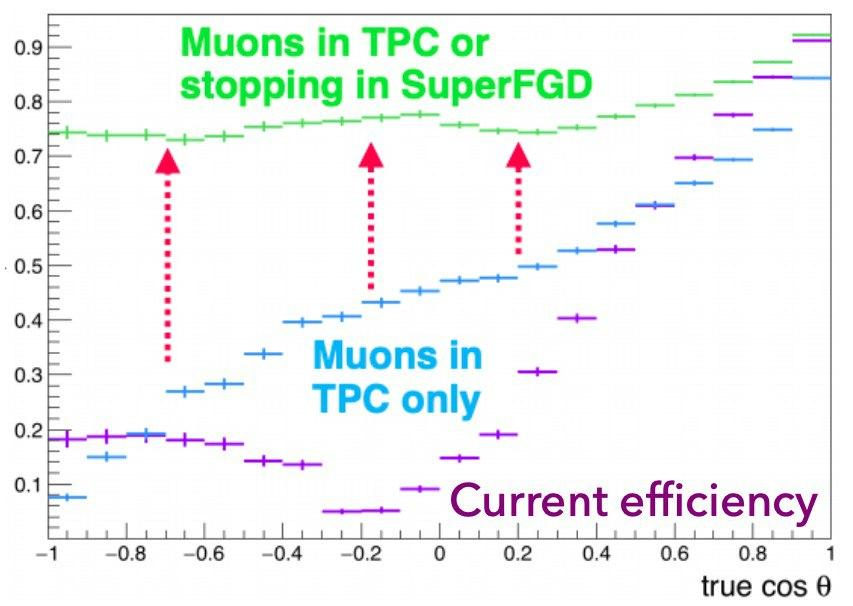
\includegraphics[width=0.5\linewidth]{new_eff}
  \caption{Efficiency of the muon detection upgraded ND280 versus the current one (in violet). The blue line represents muons that exit SuperFGD and are tracked with TPC, the green line take into account also muons contained in SuperFGD only.}
  \label{fig:up:eff_up}
\end{figure}

% efficiecny for various energy & cos theta
\begin{figure}[!ht]
  \centering
  \begin{minipage}{0.49\linewidth}
    \centering
    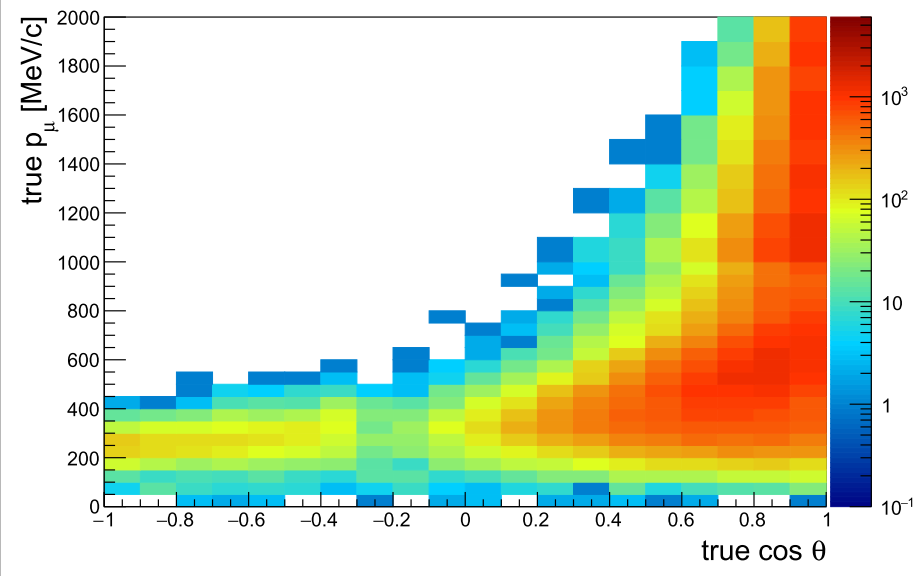
\includegraphics[width = \linewidth]{ph_old} \\ (a)
  \end{minipage}
  \begin{minipage}{0.49\linewidth}
    \centering
    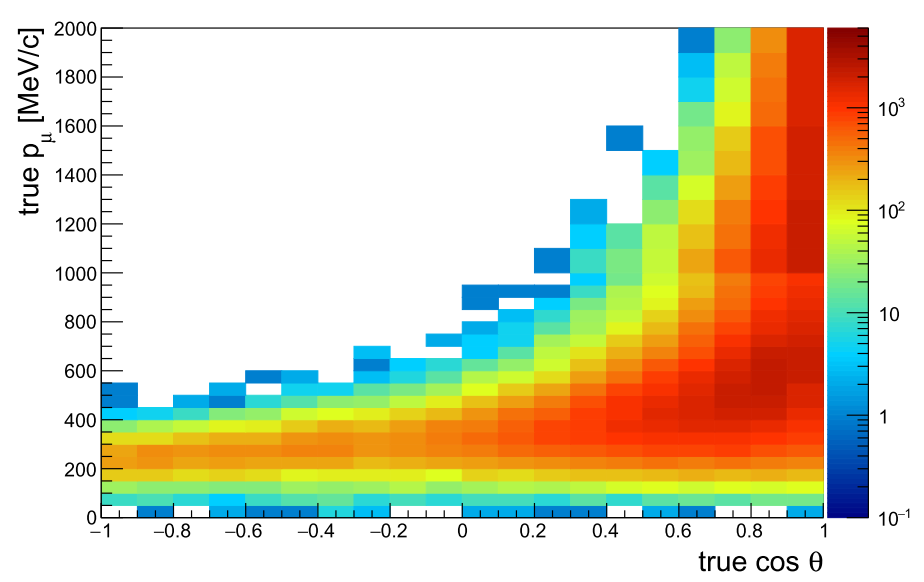
\includegraphics[width = \linewidth]{ps_up} \\ (b)
  \end{minipage}
    \caption{Muon kinematics selected from $\nu_\mu$CC interactions with current (a) and upgraded (b) configuration of the ND280.}
    \label{fig:up:phase_space}
\end{figure}




\end{document}
